For the following pool boiling curve:

\newpart{10}
Label both the X and Y axis with the proper label and units.  Label the temperatures indicated by the arrows and give a brief description of what each represents.
\iftoggle{NoFig}{
\begin{center}
         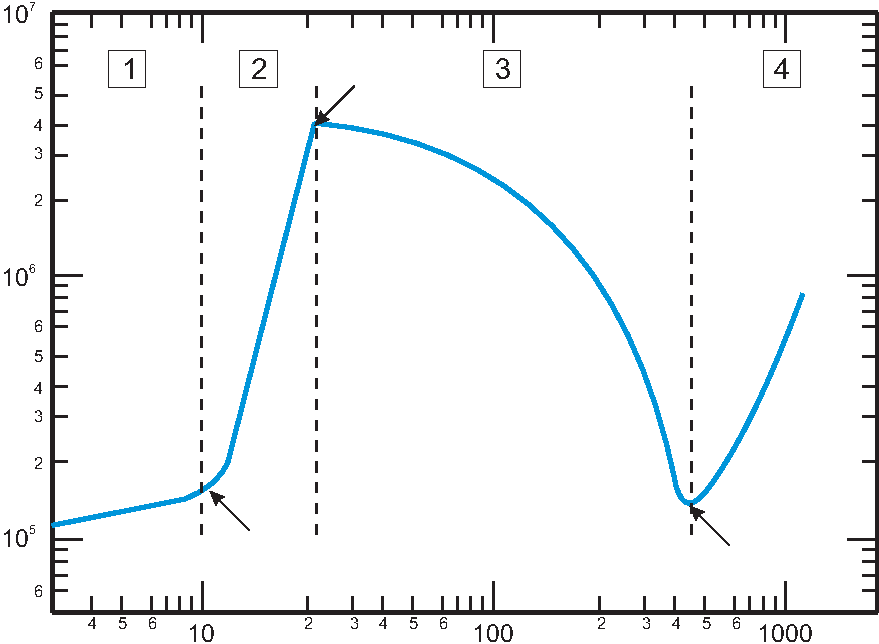
\includegraphics[width=3in]{../Figures/PoolBoiling.pdf}
\end{center}
}

%
% Solution
%
\iftoggle{Solution}{
  \vspace{12pt}
  \begin{addmargin}[1em]{2em}
    \textbf{Solution:}
    \vspace{12pt}
\begin{center}
         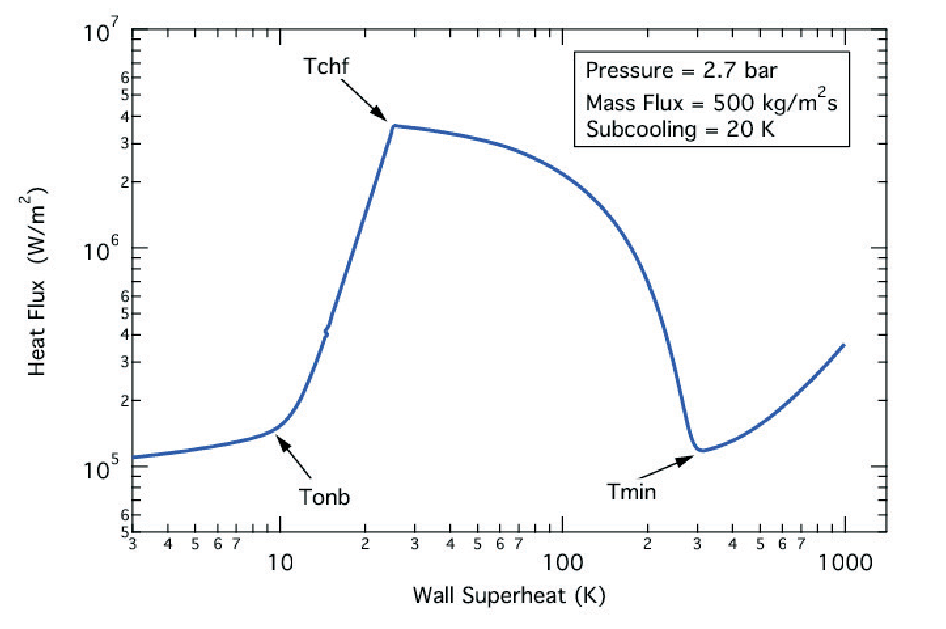
\includegraphics[width=5in]{../Figures/PoolBoilingSol.pdf}
\end{center}
    
   \end{addmargin}
}
\vfill

\newpart{5}
For each region indicated by the number 1-4 in the figure above, give the name of the region and a brief description of the boiling in that region.
%
% Solution
%
\iftoggle{Solution}{
  \vspace{12pt}
  \begin{addmargin}[1em]{2em}
    \textbf{Solution:}
    \vspace{12pt}
\begin{enumerate}
\item Convection to a single phase liquid.
\item Nucleate Boiling.
\item Transition Boiling.
\item Film Boiling.
\end{enumerate}
    
   \end{addmargin}
}
\vfill


